%Corps du document :
%\setlength{\parindent}{1cm}

\section{Objectifs}

Le but de ce projet était de réaliser un analyseur de documents XML, utilisant les outils flex et bison pour définir une grammaire et construire un parseur. Un document XML est représenté en mémoire selon une structure de donnée définie ci-après, et il peut être validé selon une DTD, dont la structure de donnée est aussi définie ci-après. Un document peut également être transformé grâce à une feuille de style XSLT.

\section{Structures de données}

Voici la description des structures de données que nous avons utilisées dans le cadre de ce projet :

\subsection{Diagrammes UML détaillés}

\subsubsection{Modèle XML}

\medskip
\begin {center}
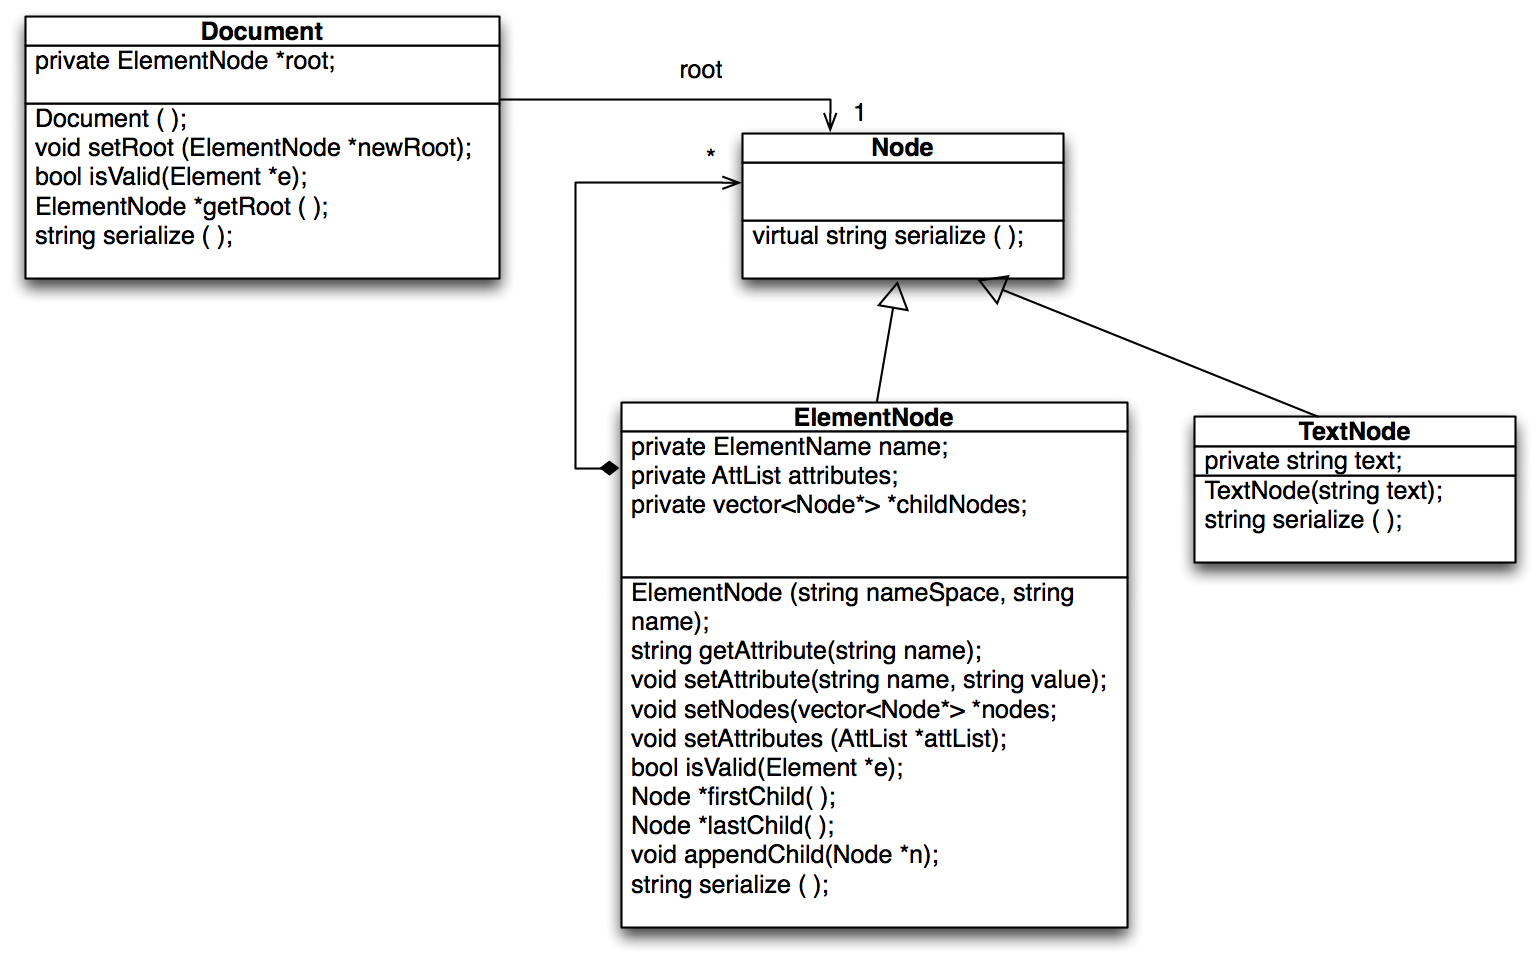
\includegraphics[width=\textwidth]{UMLXML.png}
\end {center}
\medskip

\subsubsection{Modèle DTD}

\medskip
\begin {center}
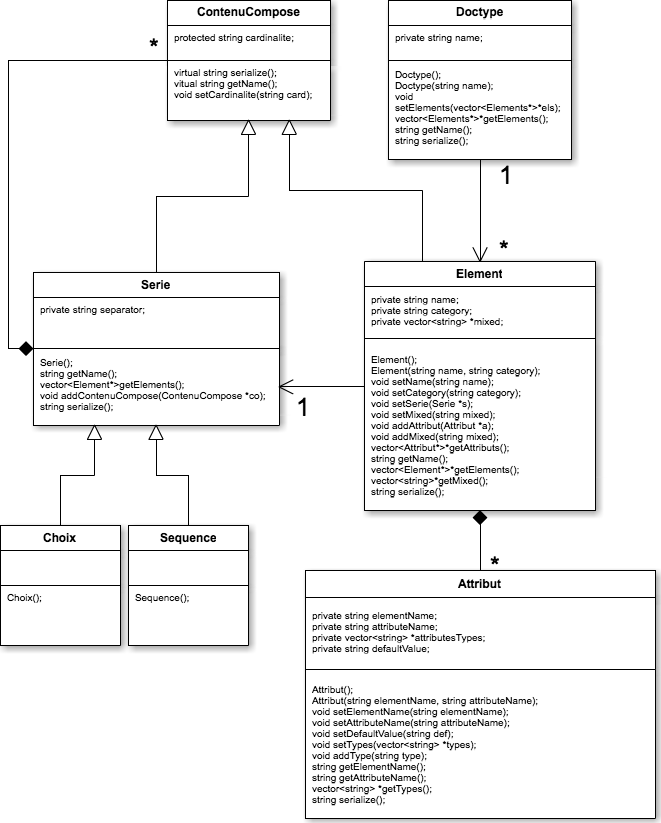
\includegraphics[width=\textwidth]{UMLDTD.png}
\end {center}
\medskip

\section{Algorithmes}

Voici les algorithmes principaux que nous avons implémenté pour effectuer la validation d'un document XML par une DTD, et pour effectuer sa transformation par rapport à une feuille de style XSLT :

\subsection{Algorithmes de Validation}

Une validation XML simple a été implémentée de manière algorithmique. Elle fonctionne en parcourant récursivement tous les noeuds d'un document XML, vérifie que chaque noeud est autorisé par la DTD, et que tous ses attributs et sous-éléments aussi :

\begin{algorithm}
\caption{Document::isValid(DocType)}
\begin{algorithmic}
\STATE $Element \leftarrow DocType$
\RETURN $noeudRacine.isValid(Element,DocType)$
\end{algorithmic}
\end{algorithm}

\begin{algorithm}
\caption{ElementNode::isValid(Element,DocType)}
\begin{algorithmic}
\IF{$ElementNode.name not equals Element.name$}
\RETURN $false$
\ENDIF
\FORALL{$ElementNode.attribut$}
\IF{$ElementNode.attribut not in Element.attributs$}
\RETURN $false$
\ENDIF
\ENDFOR
\FORALL{$ElementNode.children$}
\IF{$ElementNode.childi is ElementNode AND is not in Element.children$}
\RETURN $false$
\ENDIF
\STATE $valid \leftarrow ElementNode.child.isValid(Element.child)$
\IF{$not valid$}
\RETURN $false$
\ENDIF
\ENDFOR
\end{algorithmic}
\end{algorithm}

\subsection{Algorithmes de Transformation}

La transformation se base sur une structure XSLT, représentée par le même modèle que pour un document XML classique. L'algorithme parcoure chaque template pour essayer de l'appliquerdepuis le document XML vers le nouveau document.

\newpage

\begin{algorithm}
\caption{TransformXML(documentXML,documentXSL)}
\begin{algorithmic}
\STATE $resultat \leftarrow new Document$
\FORALL{$template$}
\IF{$template de la raçine$}
\STATE $resultat.racine \leftarrow transformTemplate(templateRacine,elementNode de documentXML$
\ENDIF
\ENDFOR
\RETURN $resultat$
\end{algorithmic}
\end{algorithm}

\begin{algorithm}
\caption{TransformTemplate(nodeXML,template)}
\begin{algorithmic}
\STATE $result \leftarrow liste de node$
\IF{$template n'a pas le namespace xsl$}
\STATE $node \leftarrow new ElementNode(nom de template,attribut de template)$
\STATE $ajout de node dans result$
\ENDIF
\FORALL{$enfant de template$}
\IF{$enfant est un ElementNode$}
\IF{$namespace de l'enfant est xsl$}
\IF{$nom de l'enfant est apply-templates$}
\IF{$un template s'applique à un enfant de nodeXML$}
\STATE $result \leftarrow TransformTemplate(enfant de nodeXML,template à appliquer)$
\ENDIF
\ELSIF{$nom de l'enfant est value-of$}
\STATE $result \leftarrow enfants de nodeXML$
\ENDIF
\ELSE
\STATE $result \leftarrow TransformTemplate(nodeXML,enfant du template)$
\ENDIF
\ELSE
\STATE $result \leftarrow enfant du template$
\ENDIF
\ENDFOR
\RETURN $result$
\end{algorithmic}
\end{algorithm}

